\subsubsection{ Дизайн веб-сайта проекта }

Трудно себе представить в современном мире компанию или программный продукт без персональной страницы в сети Интернет. В связи с этим возникла необходимость создания веб-сайта для проекта <<COEX>>.

Современные тенденции в веб-дизайне, как и в приложениях: минимализм и простота функционала. Крупнейшие корпорации в течение последних лет выпустили гайдлайны для своих продуктов: у Microsoft --- ModerUI, у Google --- Flat Design.
В качестве основного направления для дизайна выбран плоский стиль с минимум сторонней графики. Используемые технологии: HTML5, CSS3, JavaScript.
Не менее важным является структура будущего макета, для этого необходимо выделить основные блоки информации, которые будут на сайте:
\begin{enumerate}
  \item Информация о системе. Здесь необходимо описать, что представляет из себя система <<COEX>> и ее необходимость.
  \item Возможности системы, описание плагинов.
  \item Установка. Как установить систему, ссылки на скачивание.
  \item Архитектура. Информация о структуре системы.
  \item Контакты.
\end{enumerate}

Исходя из вышесказанного был выбран первый вариант макета: сайт-презентация (рис.~\ref{lo1:lo1}).

\begin{figure}[h!]
\center{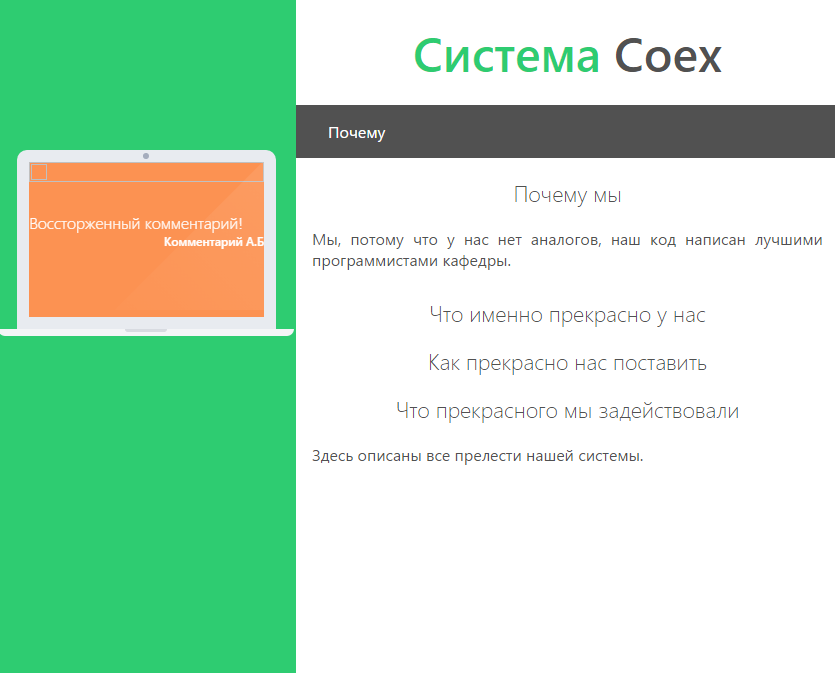
\includegraphics[width=0.7\linewidth]{lo1}}
\caption{ Первый вариант дизайна }
\label{lo1:lo1}
\end{figure}

Позднее данный дизайн был отклонён из-за нерационального использования пространства веб-страницы и сложности расположение контента в пользу нового варианта (рис.~\ref{lo2:lo2}).

\begin{figure}[h!]
\center{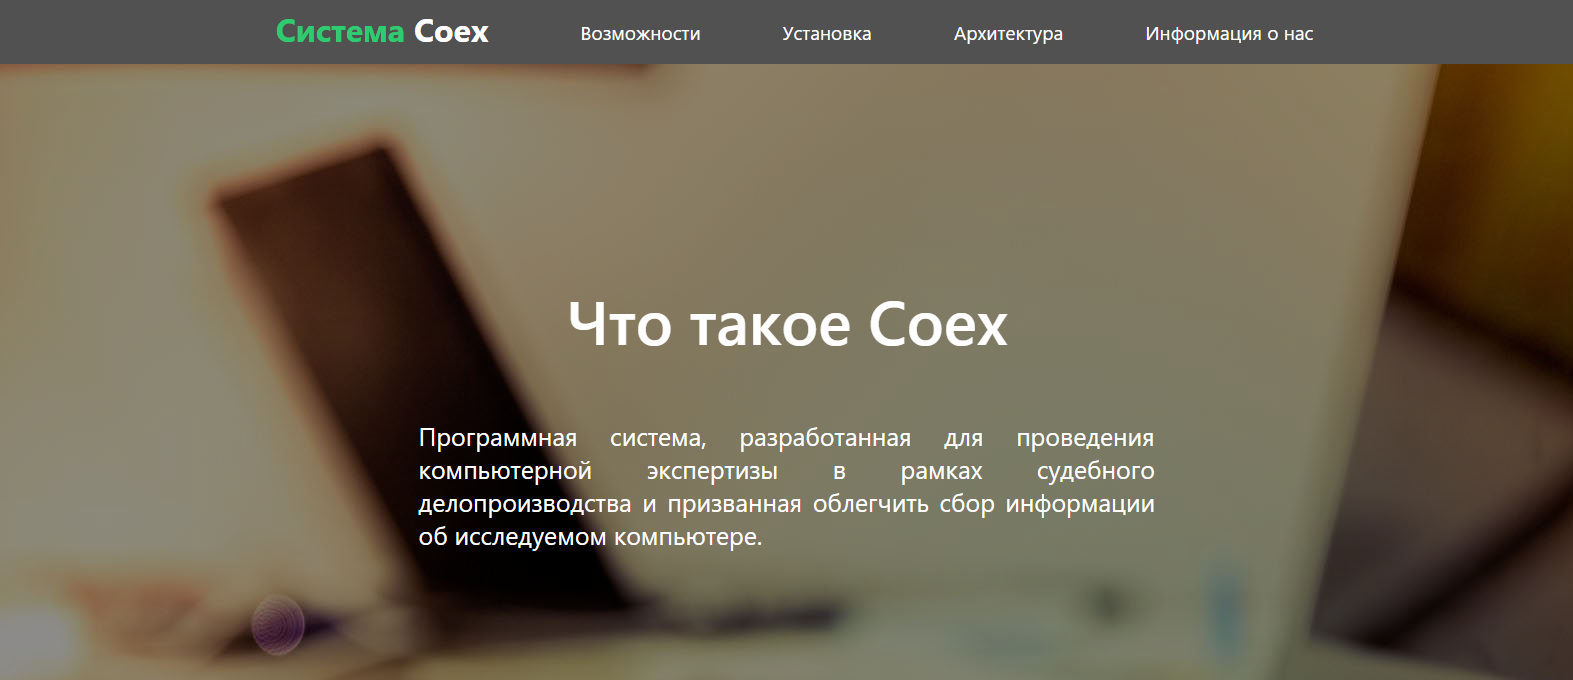
\includegraphics[width=0.8\linewidth]{lo2}}
\caption{ Новый вариант дизайна }
\label{lo2:lo2}
\end{figure}

Был выбран вариант с одним блоком информации на одну страницу <<прокрутки>> --- так можно акцентировать внимание посетителя на необходимых деталях.

\subsubsection{ Вёрстка дизайна } 

Как было сказано ранее, для верстки использовались технологии HTML5 и CSS3, что позволило существенно сократить код стилей и нагляднее писать код страницы. Минусом данного подхода является требование к наличию у посетителей последних версий интернет-браузеров, но, как показывает статистика, количество таких пользователей превалирует (рис.~\ref{lo3:lo3}).

\begin{figure}[h!]
\center{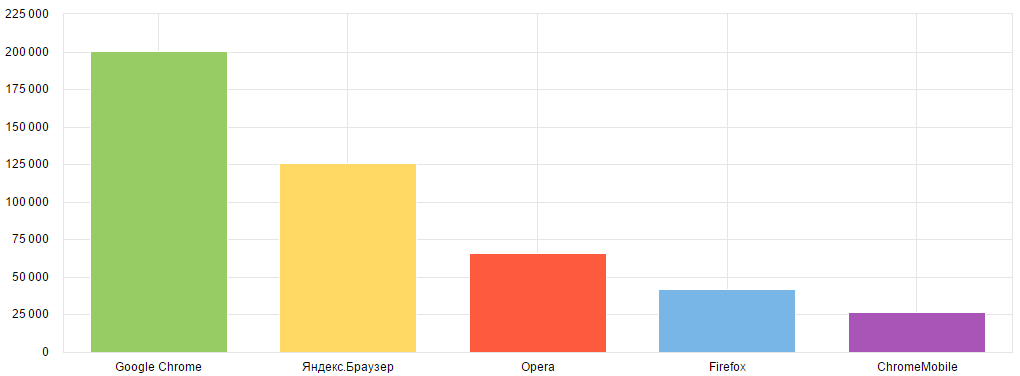
\includegraphics[width=0.8\linewidth]{lo3}}
\caption{ Количество посетителей с различными браузерами }
\label{lo3:lo3}
\end{figure}

Для обеспечения поддержки мобильных устройств и устройств с нестандартным разрешение экрана в вёрстке максимально использованы новые возможности CSS3, такие как flex-box, box-sizing и другие (рис.~\ref{lo4:lo4}).

\begin{figure}[h!]
\center{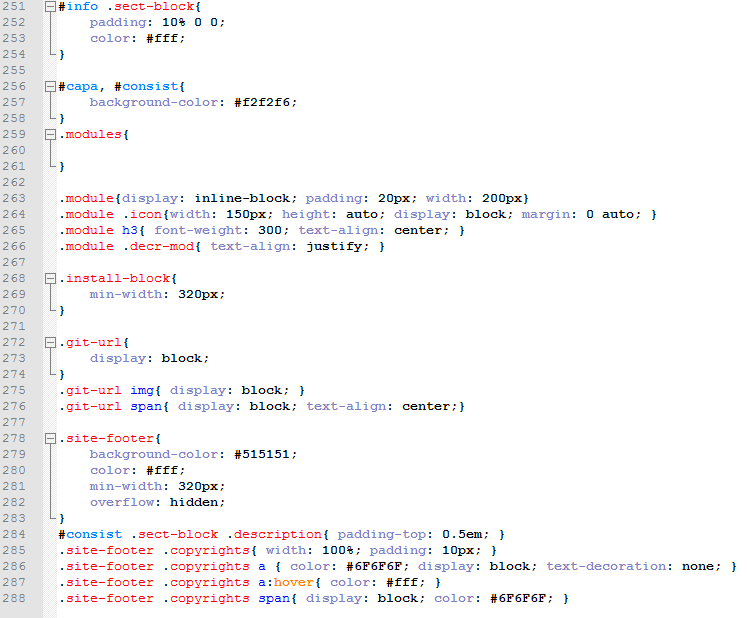
\includegraphics[width=0.8\linewidth]{lo4}}
\caption{ Часть кода CSS-стилей }
\label{lo4:lo4}
\end{figure}

\subsubsection{ Регистрация домена }

Был подобран и зарегистрирован домен coex.su, параллельно с этим изучены принципы построения DNS серверов и NX записи (рис.~\ref{lo5:lo5}).

\begin{figure}[h!]
\center{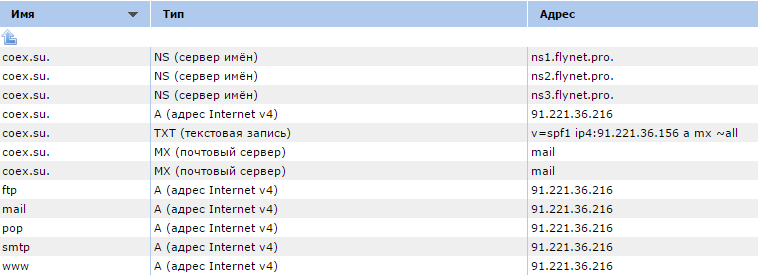
\includegraphics[width=0.8\linewidth]{lo5}}
\caption{ Пример NX-записей для домена coex.su }
\label{lo5:lo5}
\end{figure}

\subsubsection{ Настройка WEB-сервера }

Для сайта был запущен и настроен веб-сервер apache в связке с nginx. В дальнейшем apache будет <<отдавать>> посетителям динамический контент, такой как новости, а nginx – статический: исходные коды программы с репозитория, картинки, видео и прочее (рис.~\ref{lo6:lo6}).

\begin{figure}[h!]
\center{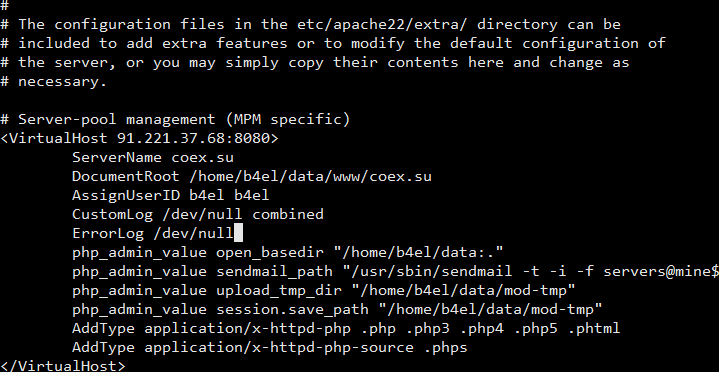
\includegraphics[width=0.8\linewidth]{lo6}}
\caption{ Часть конфига Apache }
\label{lo6:lo6}
\end{figure}

\subsubsection{ Контент }

Для наполнения сайта были написаны тексты, описывающие систему, ее части и возможности. Для каждого плагина была подготовлена своя иконка (рис.~\ref{lo7:lo7}) и описание.

\begin{figure}[h!]
\center{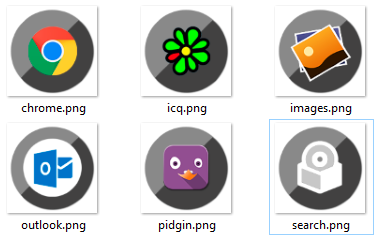
\includegraphics[width=0.7\linewidth]{lo7}}
\caption{ Иконки для плагинов }
\label{lo7:lo7}
\end{figure}

\clearpage








